\begin{figure}[h]%
    \centering%
    \begin{subfigure}{.5\textwidth}%
        \centering%
        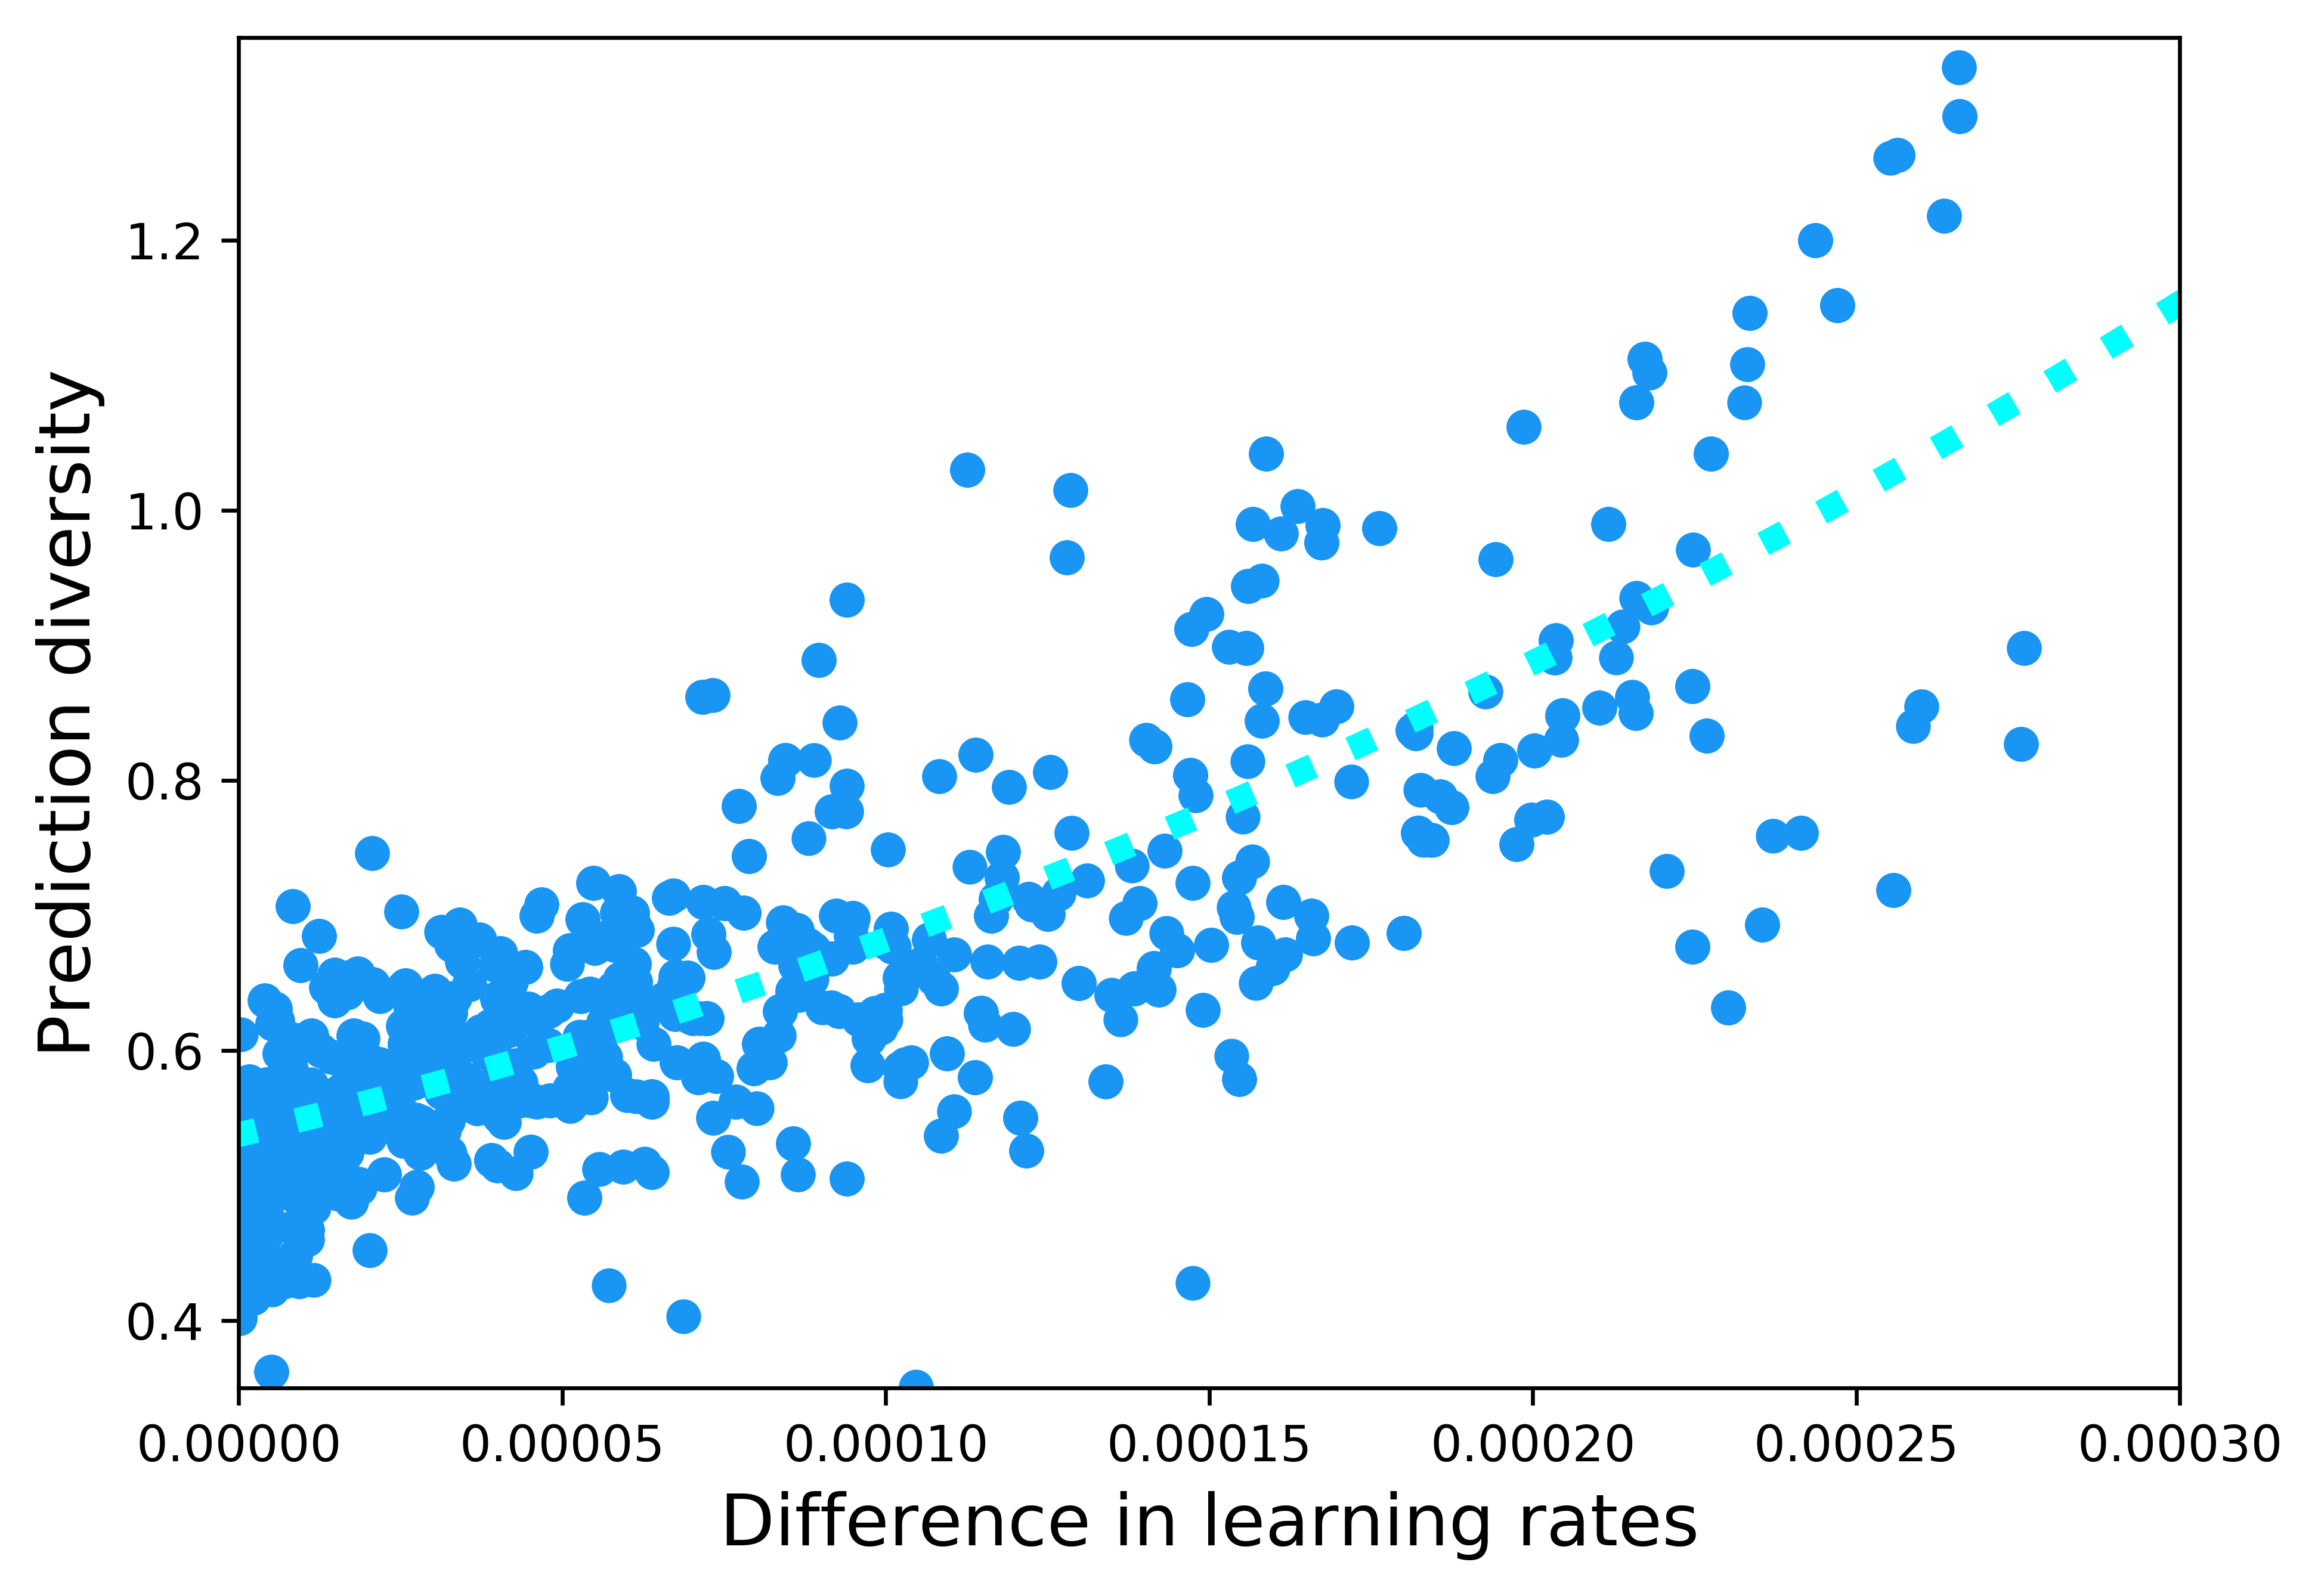
\includegraphics[width=1.0\textwidth]{pictures/files/final/diffruns_lrs_dr.png}%
        \caption{\reb{Prediction diversity ($\uparrow$) \cite{aksela2003comparison} between models.}}
        \label{fig:home0_lrs_dr}%
    \end{subfigure}%
    \begin{subfigure}{.5\textwidth}%
        \centering%
        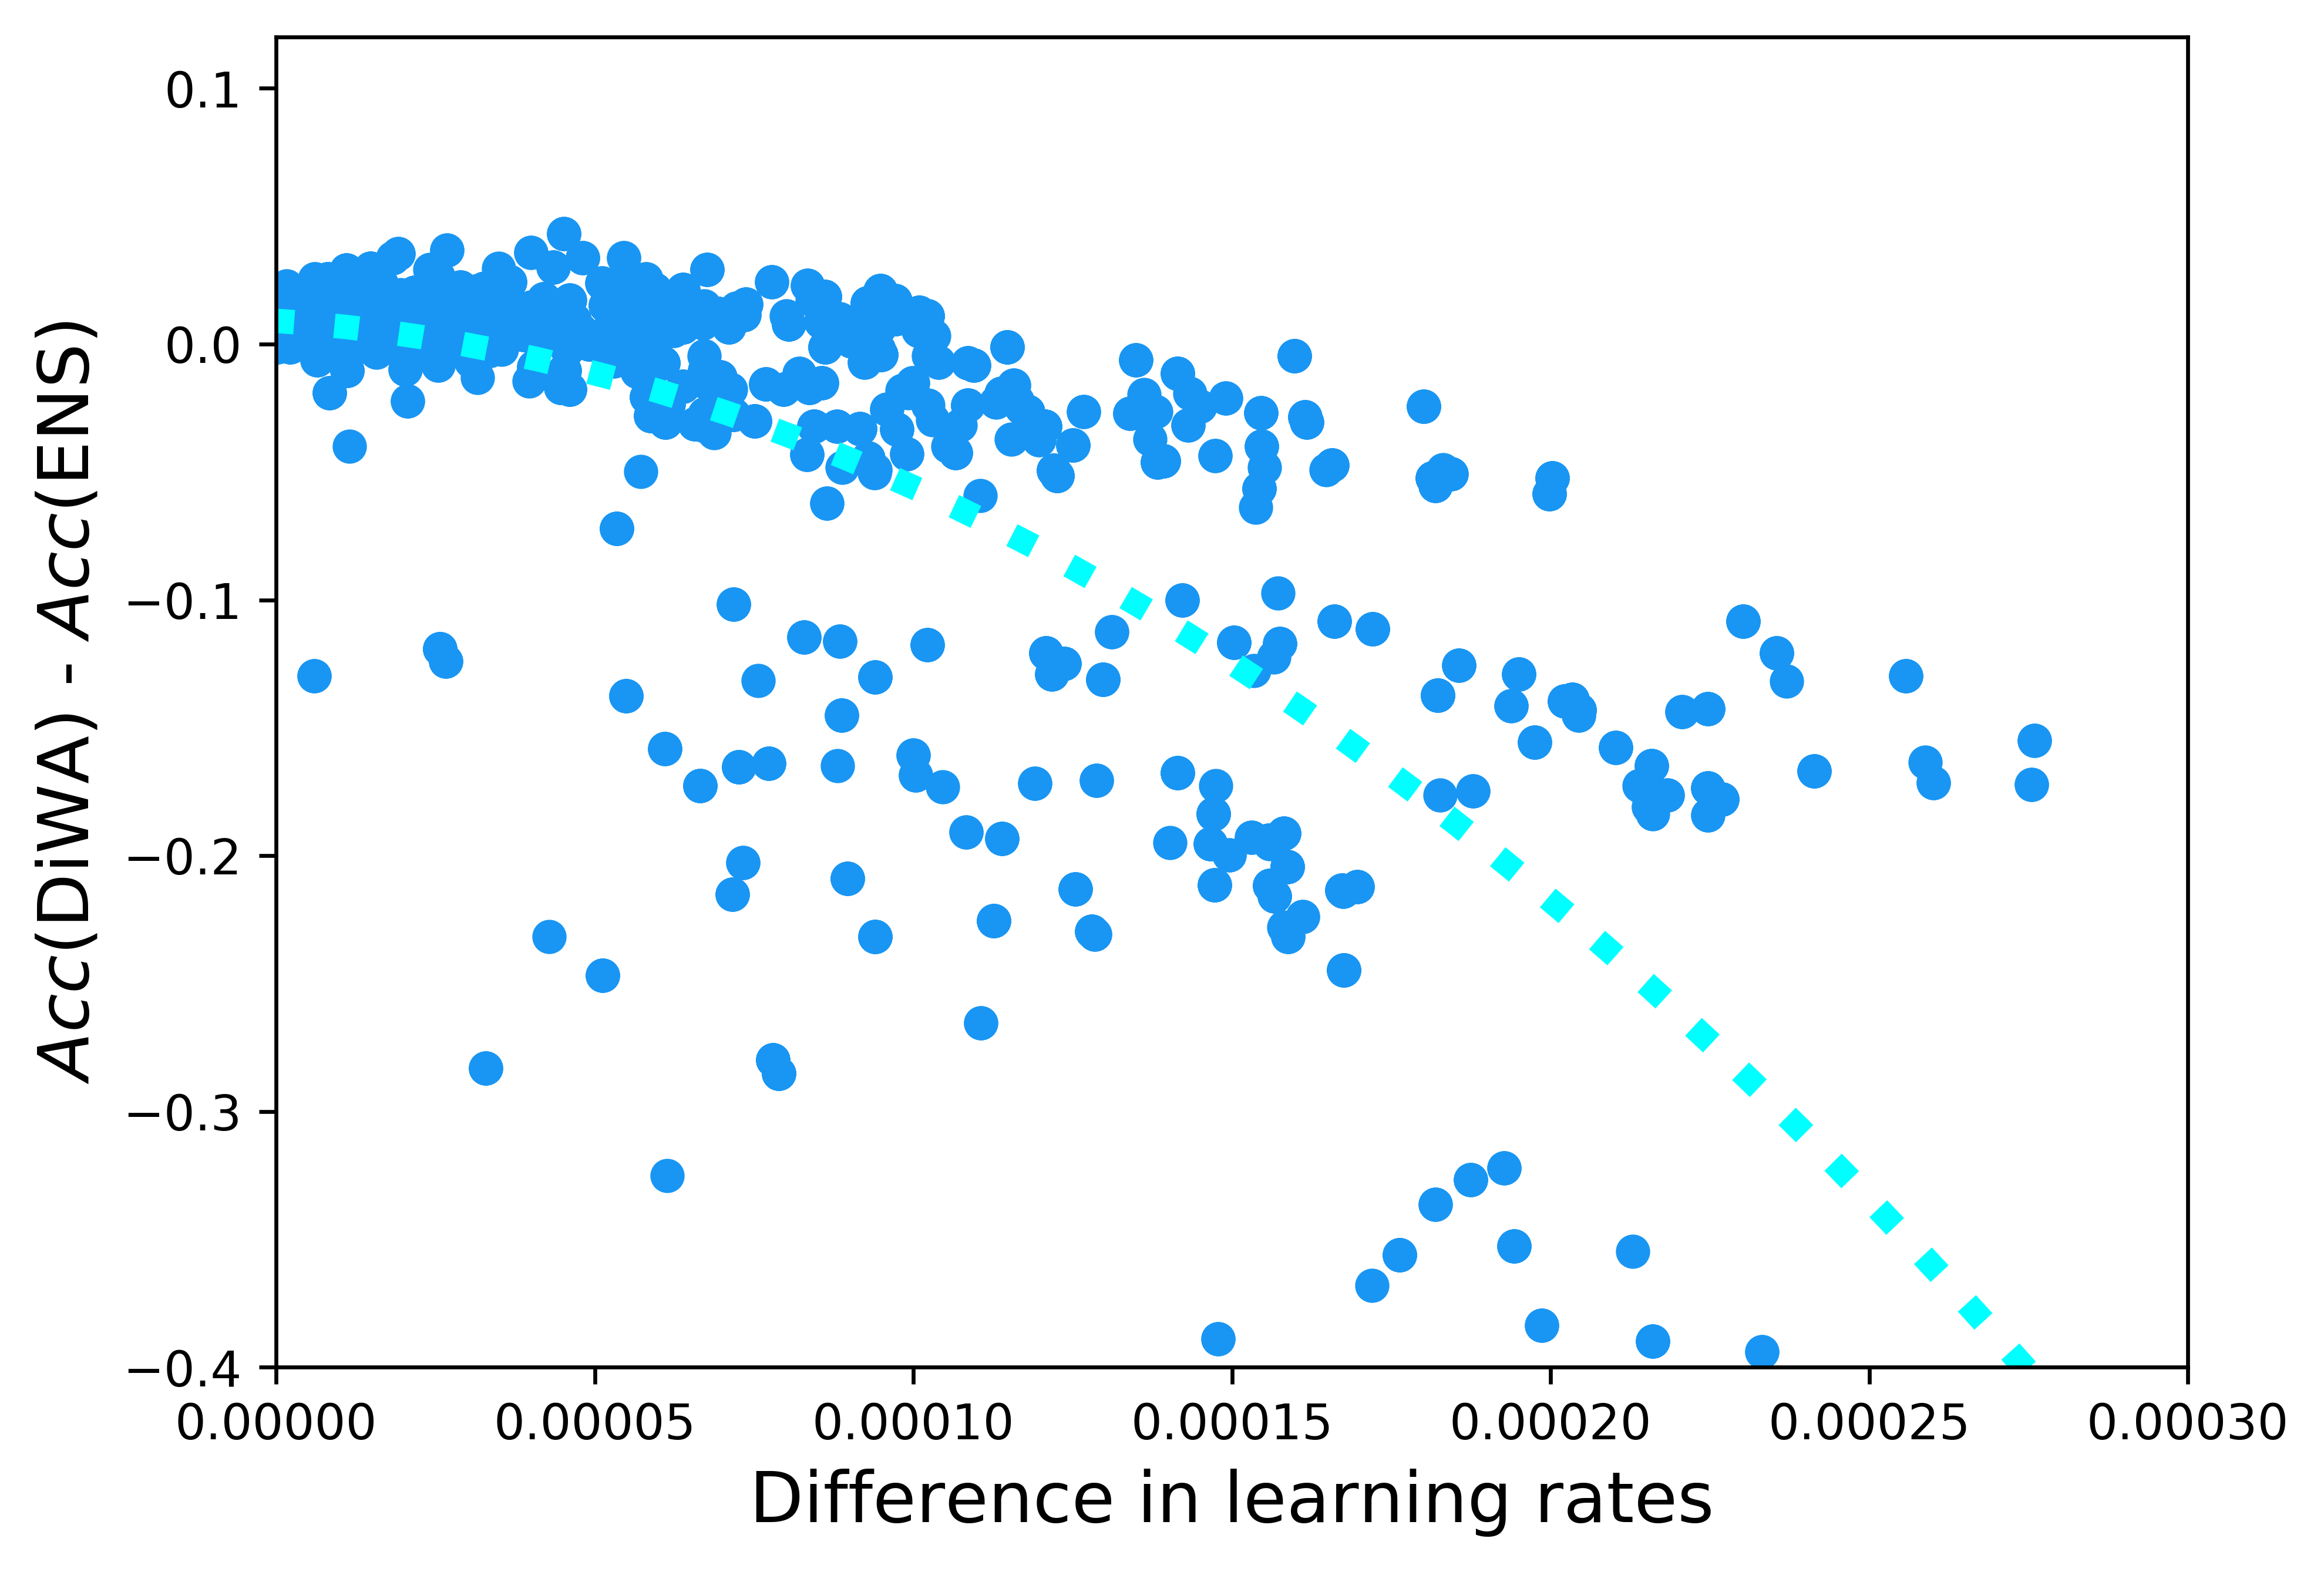
\includegraphics[width=1.0\textwidth]{pictures/files/final/diffruns_lrs_acc_net.png}%
        \caption{\reb{Accuracy ($\uparrow$) difference between DiWA and ENS.}}
        \label{fig:home0_lrs_acc}%
    \end{subfigure}%
    \caption{\reb{\textbf{Trade-off between diversity and averageability for various differences in learning rates}. Considering $M=2$ weights obtained from two learning procedures with learning rates $\text{lr}_1$ and $\text{lr}_2$ (sampled from the extreme distribution in \Cref{tab:hyperparam}), we plot in \Cref{fig:home0_lrs_dr} the prediction diversity for these $M=2$ models \versus $|\text{lr}_1-\text{lr}_2|$. Then, in \Cref{fig:home0_lrs_acc}, we plot the accuracy differences $\operatorname{Acc}(\text{DiWA})-\operatorname{Acc}(\text{ENS})$ \versus $|\text{lr}_1-\text{lr}_2|$.}}
    \label{fig:home0_lrs}%
\end{figure}%
